Many weather forecasting, assimilation, and dissemination systems are developed to reduce the damage-causing by natural disasters such as floods, storms, hurricanes, and even droughts. Other countries are also using those systems while adopting them to specific weather conditions. This chapter presents a literature review on existing systems and their architectural designs. In \cref{se:fews}, we present \acrfull{fews}, an open model integration framework. \acrfull{lead}, a distributed open data handling platform as closed-source software, is presented in \cref{se:lead}. In \cref{se:dias}, we discuss \acrfull{dias}, which is a common data platform that can manage weather data. \acrfull{madis} is another widely used data integration system, which also provides data access with quality controls is presented in \cref{se:madis}. Under each system, we explore their system architecture, scalability, and flexibility.

%%%%%%%%%%%%%%%%%%%%%%%%%%%%%%%%%%%%%%%%%%%%%%%%%%%%%%%%%%%%%%%%%%%%%%%%%%%%%%%%
\section{\acrshort{fews} flow forecasting system}
\label{se:fews}

Deltares developed \acrshort{fews} \cite{Werner2013TheSystem} in Netherland for operational forecasting agencies. The \acrshort{fews} codebase is not fully open source at the moment. The main objective of a forecasting system is to run multiple NWMs, hydrologic, and hydrodynamic models which are required for the predictions. This approach is known as a model-centric approach \cite{Werner2005FloodCatchments}. In the model-centric approach, the inputs need to be in the format specific to the model. Also, the outputs produced by the models are specific to the model; hence, difficult to integrate with other models. For example, FLO2D creates human-readable text output files. However, the Delft-FEWS uses a more modular approach, which is easier to integrate new models and redevelop the system for new requirements. Thus, Delft-FEWS is an integration framework or middleware for the models, rather specific model workflow for weather forecasting.

A forecasting flow creates a sequence of modeling steps by combining data transformation algorithms. In a forecasting flow, each step processes and feeds data into the next step. The \acrshort{fews} is flexible enough to integrate new models and algorithms into the core codebase that can be used to create new workflows \cite{Werner2013TheSystem}. So, the \acrshort{fews} framework is capable of integrating models into the system and creating workflows for forecasting.

Are proposed by Haggett \cite{Haggett1998AnWales} key elements of a forecasting system are defined as detection, forecasting, dissemination and warning, and responding to the events. The \acrshort{fews} focuses on the forecasting step out from above steps. The main objective of this step is to provide additional lead time by forecasting future hydro-meteorological conditions \cite{Werner2005FloodCatchments}. It is a valid argument that providing accurate predictions with greater lead time can reduce the level of destruction. To forecast, the system should be capable of integrating real-time data from meteorological and hydrological observation network systems, and the disseminate the forecasted results through relevant products to the warning process.

Haggett \cite{Haggett1998AnWales} summarized the key elements of a forecasting system as detection, forecasting, dissemination, and warning, and responding to the events. The \acrshort{fews} focuses on the forecasting step out above four steps. The main objective of this step is to provide additional lead time by forecasting future hydrometeorological conditions \cite{Werner2005FloodCatchments}. It is a valid argument that providing accurate predictions with more considerable lead time can reduce the level of destruction. Further, the forecasting system should be capable of integrating real-time data from weather data observation networks and disseminate the forecasted results through relevant parties to the warning process.

\cref{fi:fews_schematic} shows the connection between a forecasting system to real-time data integration systems and dissemination systems. One of the widely practiced use cases is to use meteorological forecast data to estimate precipitation, and then use a hydrological and hydraulic model chain to predict the surface water level affected. The hydrological and hydrodynamic models should design based on geographical data. The ground surface should be examined geographically and divided into catchments. Based on the affected catchment, it can be further divided into sub-catchments to reduce the complexity of the simulation task, and reduce simulation time with parallel processing. Ideally, the forecasting system flexible enough to allow modification of models and data while keeping the system interaction method constant as working with multiple forecasters.

\begin{figure}[htp]
    \centering
    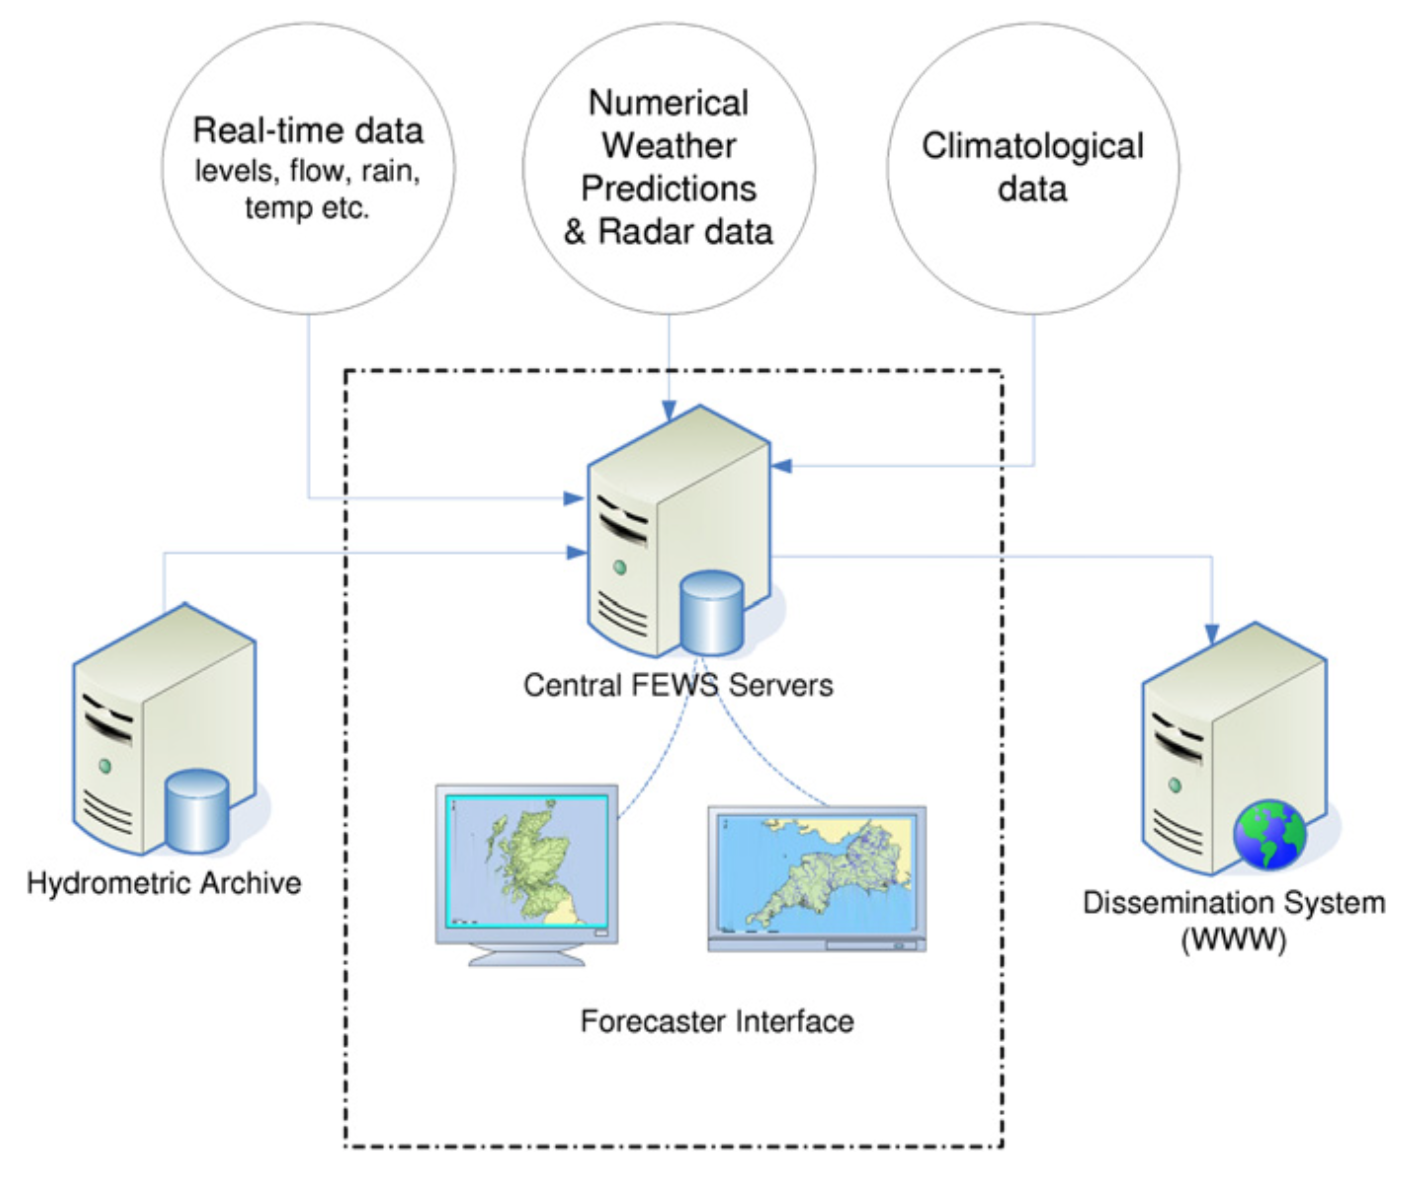
\includegraphics[width=0.8\textwidth]{lit/fews/Schematic-structure-of-a-fl-ood-forecasting-system-showing-the-position-of-Delft-FEWS_W640.png}
    \caption[Schematic structure of a flood forecasting system including \acrshort{fews} and communication among other operational systems]{Schematic structure of a flood forecasting system including \acrshort{fews} and communication with other operational systems \cite{Werner2013TheSystem}.}
    \label{fi:fews_schematic}
\end{figure}

The \acrshort{fews} follows a data-centric approach, where it provides a common data-model to interact with other components. All the timeseries data stored in a database by converting them to a common data model. New models are integrated into the system by using one of the interfaces provided to interact with the common data-model \cite{Werner2013TheSystem}. The common data-model allows storing data efficiently without duplicates. Then, the system supports operations like creating forecast reports and sharing the data by integrating new codebase as adapters. However, this approach cannot handle multiple data formats. The \acrshort{fews} overcome this issue by introducing adapters for most of the commonly used data formats such as CSV, NetCDF, and JSON. While this enables users to import data into the system; it also introduces adding additional complexity to the system.

The timeseries data is one of scalar, vector, or grid data type. And different types of data stored as binary objects in a timeseries table inside the \acrshort{fews} system. Functional components or any integrated models do not have direct access to the timeseries table, and those should use the data access module to access the data \cite{Werner2013TheSystem}. As explained in the system interpretation, all data access requests need to go through the data access module cause to increase the cost of data access. Because the \acrshort{fews} stores different data types as binary objects, there is a penalty for converting data into binary objects and vice versa. Since all timeseries data is stored within a single data source, it allows the system to handle data without much system complexity. However, a single data source becomes a bottleneck when it is required to fulfill all the timeseries data requirements. Further, the performance goes down due to the need to scream Spatio-temporal weather data.

Given the above drawback on storing the data in the system, the Delft-FEWS data model uses a set of primary attributes from weather data to identify a timeseries uniquely. Those primary attributes are location, data type, and source of the data \cite{Werner2013TheSystem}. The primary attributes are always required, and there are some secondary attributes to add timeseries metadata further. Also, primary attributes used to index data for making data queries faster. Moreover, Delft-FEWS is able to create separate indexes for each attribute while storing large amounts of data. As an example, the system can separate timeseries data into multiple databases based on the source of timeseries, such as an external source of data or a hydrological model, which creates the timeseries and then index each database on other attributes. Alternatively, separate timeseries by data type and stored in multiple storages give the capability for the system to scale with a factor of identical types. An example of separation by data types of scalar, vector, and gridded will increase the scaling factor by 3x.

Data preprocessing and manipulation are necessary processes in weather forecasting. The data integrated from external sources are not in the appropriate temporal and spatial format that can directly feed as an input to forecasting models or use in other applications. Therefore, the forecasting environment provides generic data processing steps to convert data into model compatible formats. Such examples are serial and spatial interpolation, data validation, aggregation and disaggregation, and data fusion \cite{Werner2013TheSystem}. This is a vital feature in a forecasting system and affects the quality and accuracy of the predicted data outputs. Because of the common data model concept in the Delft-FEWS, data processing via these functions are much useful. The system contains a set of default data processing functions, but required algorithms can implement as a new Java class integrated with the \acrfull{api} provided by the Delft-FEWS. The Delft-FEWS has language dependency while additional features integration since users need to implement the new functional extensions using Java. 

\begin{figure}[htp]
    \centering
    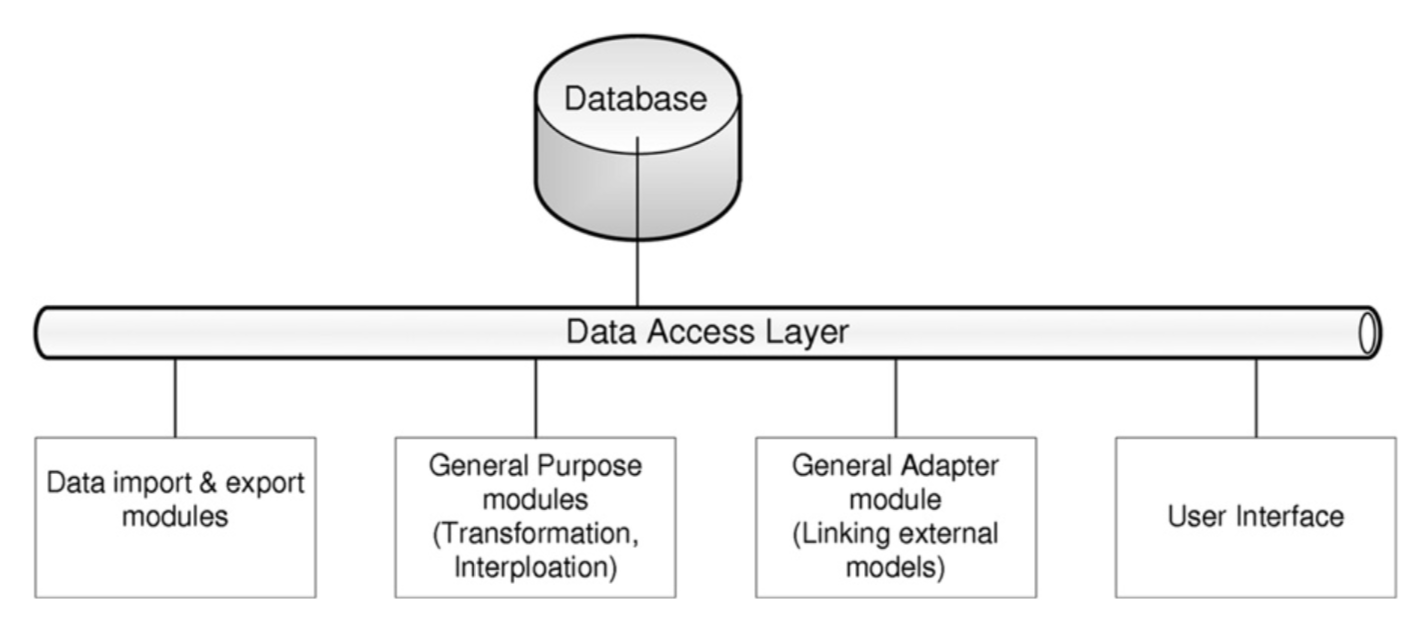
\includegraphics[width=1.0\textwidth]{lit/fews/Architecture-of-Delft-FEWS-showing-the-data-base-the-data-access-layers-and-examples-of_W640.png}
    \caption[Architecture of \acrshort{fews}]{Architecture of \acrshort{fews} \cite{Werner2013TheSystem}.}
    \label{fi:fews_data_layer}
\end{figure}

Delft-FEWS provides data processing and modeling libraries to access scalar and grid timeseries using the same method. However, the database access only allows through the data access layer, as shown in \cref{fi:fews_data_layer} \cite{Werner2013TheSystem}. The system depends on a single database instance, and all the requests are coming to the database through the data access layer. It is possible to setup and connect to an enterprise-level database with clustering and shading as a paid solution to enhance the throughput. Still, the design itself inherently suffers from a single database bottleneck when accessing a large set of timeseries by the models.

\begin{figure}[htp]
    \centering
    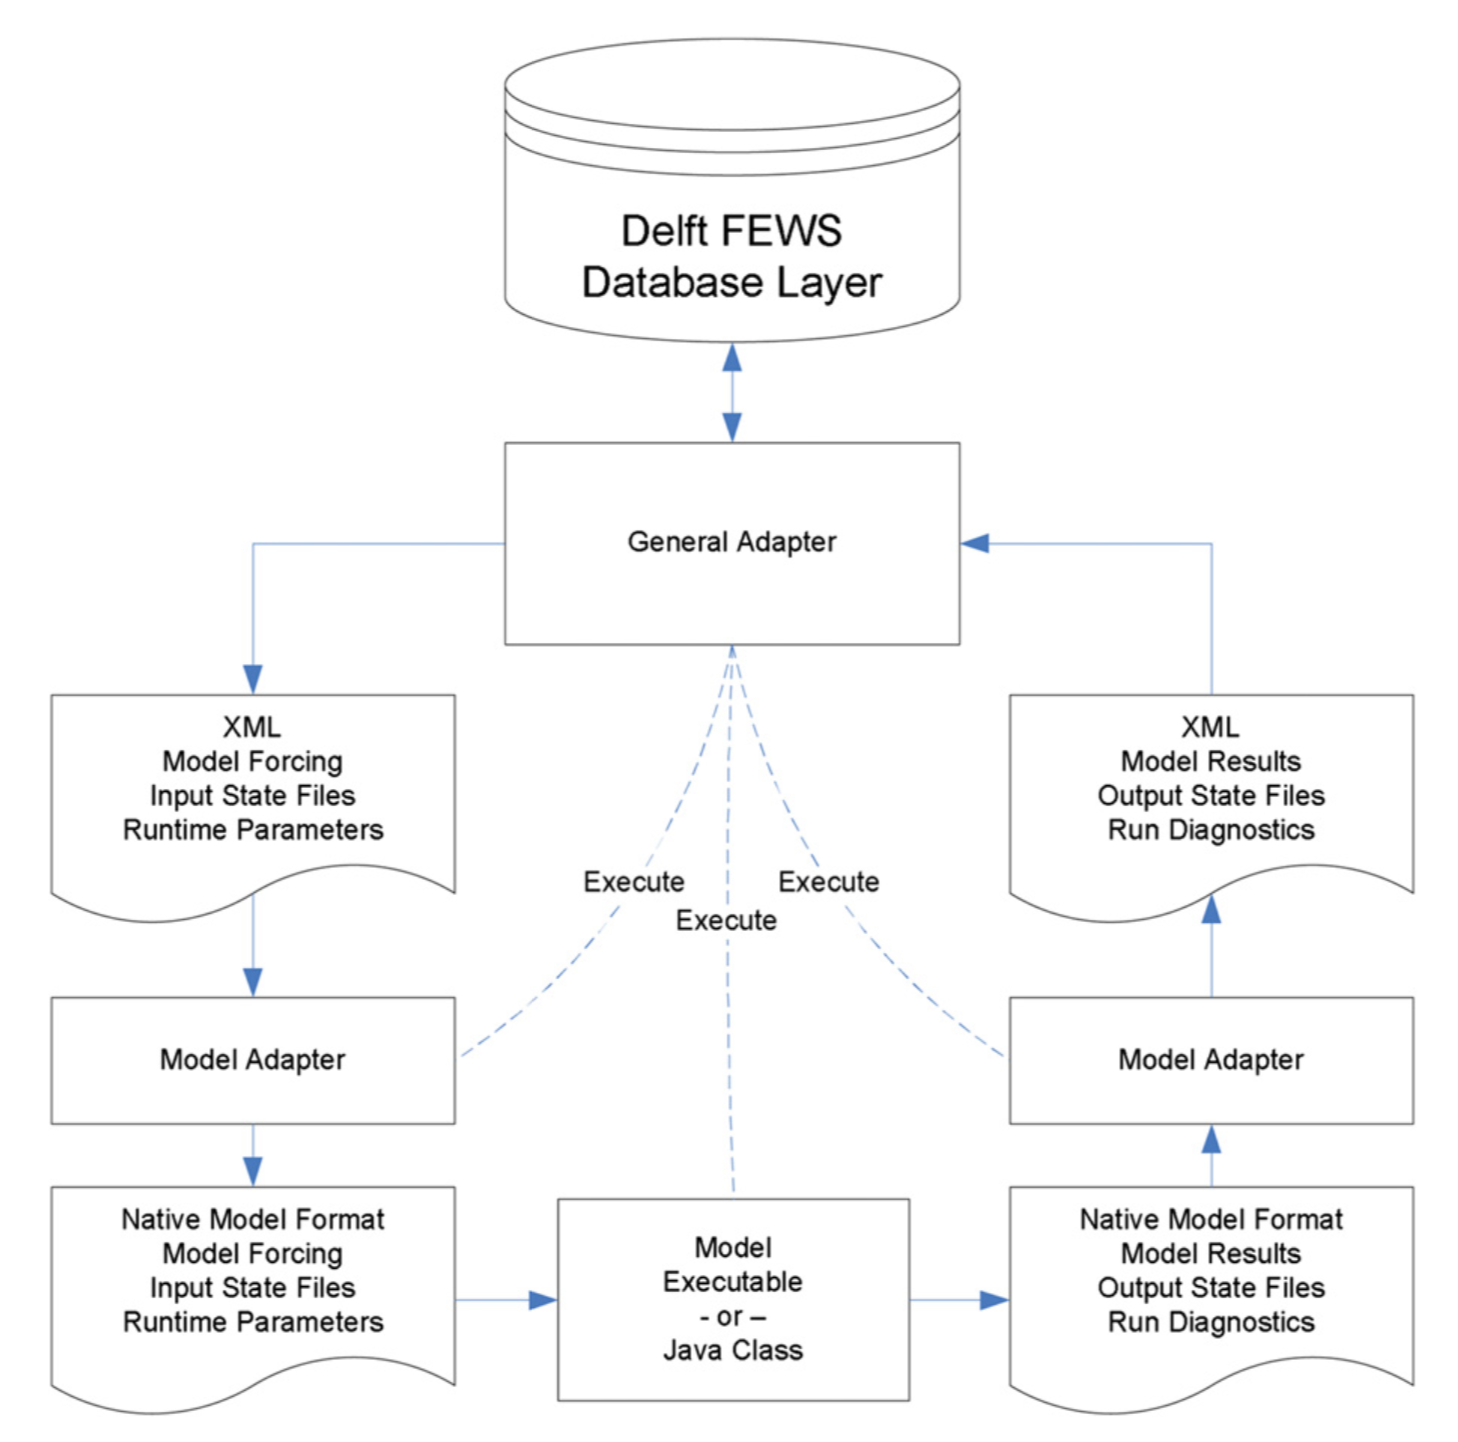
\includegraphics[width=0.9\textwidth]{lit/fews/Linking-Delft-FEWS-with-external-models-The-fi-gure-shows-the-fl-ow-of-data-through-XML_W640.png}
    \caption[\acrshort{fews} integration with external models]{Integrating \acrshort{fews} with external models \cite{Werner2013TheSystem}.}
    \label{fi:fews_general_adapter}
\end{figure}

One of the simple and most useful features in the Delft-FEWS is the use of an open approach to integrate models and data. The concept of the open modeling framework is used by the Delft-FEWS, which is proposed by open model integration \cite{Kokkonen2003InterfacingXML}. It merely gives the flexibility to allow operators to integrate more models as well as variations of the same model and come up with new forecasting flows as much as possible.

The users need to configure the input timeseries data via XML configurations, and Delft-FEWS generates the model input data as XML files. As shown in \cref{fi:fews_general_adapter}, a model adapter transforms the data into the required format for the model as a preprocessing step. The Delft-FEWS has prebuilt a set of model adapters, and users can use available model adapters. Next, the Delft-FEWS executes the external model, which generates the model output, and allows users to run multiple models parallel or run those sequentially as needed. In the post-processing step, the results of the model transform into an XML file, which imports into the database through the data access layer, as shown in \cref{fi:fews_general_adapter} \cite{Werner2013TheSystem}. The general adapter used by the Delft-FEWS for the model execution is causing tide coupling into the execution process in the system. Users do not have the flexibility to run the models with different configurations, such as parallel execution of a particular model. Those issues may be overcome by triggering an external process at the execution time. But, it introduces more difficulty in handling the next step in the forecasting flow, after the successful execution of the model. 

In this research, we do not focus on implementing workflow management, and the user has to come up with their flow mechanism or use an existing scientific flow management system. However, it is a concept that needs to be discussed and understood properly to design a data integration and assimilation system. However, the proposed architecture within the research should be capable of integrating workflow mechanisms with its extendable architecture.

The Delft-FEWS exchanges data with the models using XML files. Thus, it causes XML files to become very large when trying to access a large set of data, which can lead to I/O bottlenecks and causing performance problems \cite{Werner2013TheSystem}. The authors of the Delft-FEWS \cite{Werner2013TheSystem} seem to have noticed and accepted this problem. To overcome the issue mentioned above, they have introduced a file-based exchange of data. The proposed solution includes the use of binary XML files, the streaming of files via memory, and the use of netCDF files. Nevertheless, as far as for the users, it seems to be adding more complexity and context to get higher performance via the system.

If the user is unable to find a model adapter among available Delft-FEWS adapters, then the user has to implement the adapter for the model. The user has the flexibility to create a new adapter within Delft-FEWS, but the effort required to develop an adapter for a model will vary depending on the complexity of the data formats required by the model \cite{Werner2013TheSystem}. If the users want to use an existing adapter and need to configure something not supported via the existing adapter, it is difficult without technical support since source code is not available. Also, there are some cases it is hard to develop an adapter or running alongside the Delft-FEWS. For example, the FLO2D model used for hydrologic modeling only runs on the Windows platform. If the user sets up the Delft-FEWS on a Linux platform and uses Linux based model adapters, it is hard for users to develop a solution for integrating the FLO2D model.
